\documentclass[conference]{IEEEtran}
\IEEEoverridecommandlockouts
\usepackage{cite}
\usepackage{amsmath,amssymb,amsfonts}
\usepackage{algorithmic}
\usepackage{graphicx}
\usepackage{textcomp}
\usepackage{xcolor}
\usepackage{tikz}
\usetikzlibrary{shapes.geometric,arrows.meta,positioning,fit,backgrounds,calc}
\usepackage{booktabs}
\usepackage{multirow}

\def\BibTeX{{\rm B\kern-.05em{\sc i\kern-.025em b}\kern-.08em
    T\kern-.1667em\lower.7ex\hbox{E}\kern-.125emX}}

%-- TikZ shared styles --%
\tikzset{
  W/.style={draw, rectangle, rounded corners=3pt, align=center,
            font=\footnotesize, minimum width=6.5cm,
            text width=6.2cm, inner sep=5pt, line width=0.7pt},
  H/.style={draw, rectangle, rounded corners=3pt, align=center,
            font=\footnotesize, minimum width=2.8cm,
            text width=2.6cm, inner sep=4pt, line width=0.7pt},
  SA/.style={-{Stealth[length=2.5mm]}, thick},
  DA/.style={-{Stealth[length=2mm]}, thick, dashed, color=gray!60}
}

\begin{document}

\title{Multi-task Neuro-Symbolic Graph Neural Networks for\\Ethereum Fraud Detection with Generative Feature Augmentation}

\author{\IEEEauthorblockN{Duong Luong Minh}
\IEEEauthorblockA{\textit{School of Information and Communication Technology} \\
\textit{Hanoi University of Science and Technology}\\
Hanoi, Vietnam \\
Email: Duong.LM251038M@sis.hust.edu.vn}
}

\maketitle

%-------------------------------------------------------------------
\begin{abstract}
Fraud detection on the Ethereum blockchain involves two interrelated
challenges: identifying Ponzi schemes that exploit smart Contract
Accounts~(CA) and detecting phishing scams that target Externally
Owned Accounts~(EOA). Existing methods treat these tasks
independently, forgoing the shared graph-level semantics that underlie
both fraud patterns and struggling with severe class imbalance.
We propose \textbf{UnifiedHMSL}, a unified multi-task heterogeneous
Graph Neural Network (GNN) that simultaneously addresses both fraud
types within a single shared architecture.
Our framework introduces three innovations:
\textit{(i)} a pre-trained Conditional Variational Autoencoder (CVAE)
that generates stochastic multi-view node-feature augmentations to
alleviate class imbalance;
\textit{(ii)} a Cross-Path Attention (CPA) module enabling mutual,
gated information exchange between a generative CVAE-based
representation path and a contrastive raw-feature-based path; and
\textit{(iii)} a neuro-symbolic Expert Rules module that injects
domain-specific on-chain fraud heuristics into the learning pipeline.
These components are unified by a task-conditioned gate that learns
separate feature-blending strategies per node type (CA for Ponzi,
EOA for phishing), and trained with a joint objective combining
cross-entropy, triplet contrastive, and knowledge-guided expert losses.
Experiments on real Ethereum transaction graphs demonstrate that
UnifiedHMSL outperforms both single-task baselines and prior
multi-task approaches, confirming the benefit of unified learning with
generative augmentation and symbolic prior knowledge.
\end{abstract}

\begin{IEEEkeywords}
Fraud Detection, Ethereum, Heterogeneous Graph Neural Networks,
Multi-task Learning, Neuro-Symbolic AI, Variational Autoencoder,
Contrastive Learning, Blockchain Security.
\end{IEEEkeywords}

%-------------------------------------------------------------------
\section{Introduction}
\label{sec:intro}

Ethereum is the world's largest programmable blockchain, hosting
billions of dollars in daily transaction volume across millions of
smart contracts and user accounts.  Its open, permissionless design
has simultaneously made it an attractive target for financial fraud.
Two dominant threat categories operate at scale:
\textit{Ponzi schemes} embedded in smart contracts and
\textit{phishing scams} targeting user wallets.

Ponzi schemes on Ethereum are implemented as Contract Accounts
(CA)---addresses whose behaviour is governed by immutable
bytecode---that mimic investment platforms, redistributing funds from
later participants to earlier ones while siphoning value for the
deployer~\cite{chen2018detecting}.
Phishing attacks target Externally Owned Accounts (EOA)---user wallets
controlled by a private key---through social engineering, malicious
links, or impersonation designed to steal credentials or
funds~\cite{wu2020phishing}.

Detecting both fraud types on the Ethereum transaction graph poses three
intertwined challenges.
\textbf{First}, CA and EOA nodes interact through six heterogeneous
transaction channels (function calls and value transfers in both
directions), demanding models capable of heterogeneous message passing.
\textbf{Second}, fraud instances are severely underrepresented:
Ponzi contracts make up fewer than $15\%$ of all CA nodes and phishing
accounts fewer than $45\%$ of EOA nodes, making naive classification
prone to majority-class bias.
\textbf{Third}, existing systems treat Ponzi and phishing detection as
fully independent tasks~\cite{chen2021smartcontract,wu2020phishing},
ignoring the shared graph-level transaction semantics that underlie
both fraud patterns and doubling deployment overhead when both
detectors run simultaneously.

Graph Neural Networks (GNNs) have shown strong promise for fraud
detection in financial transaction graphs~\cite{liu2021fraud}, but
heterogeneous and multi-task extensions remain underexplored in the
blockchain security domain.  Meanwhile, generative data
augmentation~\cite{zhao2021graphsmote} and neuro-symbolic
integration~\cite{garcez2022neurosymbolic} offer complementary
avenues for addressing imbalance and improving interpretability, yet
have not been jointly applied to the Ethereum fraud detection problem.

This paper proposes \textbf{UnifiedHMSL} (Unified Heterogeneous
Multi-view Self-supervised Learning), which extends the single-task
HMSL baseline~\cite{paper_baseline_2408.00641} to a unified
multi-task framework.  Our contributions are:

\begin{enumerate}
\item \textbf{Unified multi-task architecture} with dual classification
  heads for simultaneous Ponzi~(CA) and phishing~(EOA) detection,
  jointly trained on a shared heterogeneous graph encoder to exploit
  common transaction graph structure.

\item \textbf{Cross-Path Attention (CPA)}: a mutual, gated attention
  module enabling bidirectional information exchange between a
  generative (CVAE-augmented) path and a contrastive
  (raw-feature) path, allowing each path to selectively absorb
  complementary information from the other.

\item \textbf{Task-Conditioned Gate (TCG)}: a learnable,
  per-node-type gate that dynamically blends generative and
  contrastive representations based on raw feature context, enabling
  separate fusion strategies for Ponzi~(CA) and phishing~(EOA) tasks.

\item \textbf{Neuro-Symbolic Expert Rules}: domain-specific on-chain
  fraud heuristics injected either as explicit feature channels or as
  auxiliary supervision signals, grounding the model's predictions in
  known transaction anomaly patterns.
\end{enumerate}

%-------------------------------------------------------------------
\section{Related Work}
\label{sec:related}

\subsection{Fraud Detection in Ethereum}
Early fraud detection approaches relied on hand-crafted features
extracted from bytecode or transaction metadata fed into classical
classifiers such as random forests and XGBoost~\cite{chen2018detecting}.
While effective on small curated datasets, these methods do not
generalise to the evolving structural patterns of the transaction graph.
Later work introduced opcode-frequency statistics combined with
account-level features for Ponzi contract
classification~\cite{chen2021smartcontract}.

For phishing, \cite{wu2020phishing} proposed constructing transaction
subgraphs centred on suspicious accounts and applying graph
convolutional classification.  \cite{lin2022phishing} extended this
with temporal transaction features to improve detection of recently
deployed phishing accounts.
Both lines of work target a single fraud type and do not model the
joint CA--EOA heterogeneous structure of the full Ethereum transaction
graph.

\subsection{Graph Neural Networks for Transaction Graph Analysis}
GNNs have become the dominant approach for fraud detection in
financial networks due to their ability to propagate contextual
information across multi-hop
neighbourhoods~\cite{liu2021fraud}.
\cite{dou2020commdetect} introduced a graph attention network with
camouflage suppression for social network fraud.
For heterogeneous graphs, the Heterogeneous Attention Network
(HAN)~\cite{wang2019heterogeneous} introduced meta-path-based
attention, enabling selective aggregation over multiple semantic
relation types.

The Heterogeneous Multi-view Self-supervised Learning
(HMSL) model~\cite{paper_baseline_2408.00641} most directly
underpins this work.  HMSL combines CVAE-based view augmentation
with heterogeneous message passing and contrastive self-supervision,
achieving state-of-the-art results on single-task Ponzi and phishing
benchmarks.  Our work extends HMSL to the multi-task setting and
augments it with Cross-Path Attention and neuro-symbolic expert rules.

\subsection{Multi-task Learning on Graphs}
Multi-task GNNs jointly optimise multiple task objectives over a shared
graph encoder, enabling positive knowledge transfer between related
tasks~\cite{standley2020tasks}.
In financial fraud, \cite{zheng2021fraud} demonstrated that jointly
modelling multiple fraud types in e-commerce graphs improves macro-F1
over single-task baselines.
To our knowledge, UnifiedHMSL is the first framework to apply
multi-task heterogeneous GNNs to dual Ethereum fraud detection.

\subsection{Generative Augmentation for Imbalanced Graphs}
Class imbalance is pervasive in fraud detection benchmarks.
GraphSMOTE~\cite{zhao2021graphsmote} addresses this by oversampling
minority-class nodes in the graph embedding space.
CVAE-based augmentation~\cite{li2022graphvae} generates synthetic
node features conditioned on neighbourhood context, improving
minority-class representation without distorting the graph topology.
Our ICVAE module follows this paradigm, conditioning generation on
source node features \textit{and} edge type, producing $K$ stochastic
views per node that serve as anchor, positive, and negative samples
for contrastive self-supervision.

%-------------------------------------------------------------------
\section{Proposed Methodology}
\label{sec:methodology}

%----- FIGURE 1: Overall Architecture (spans both columns) -----------
\begin{figure*}[t]
\centering
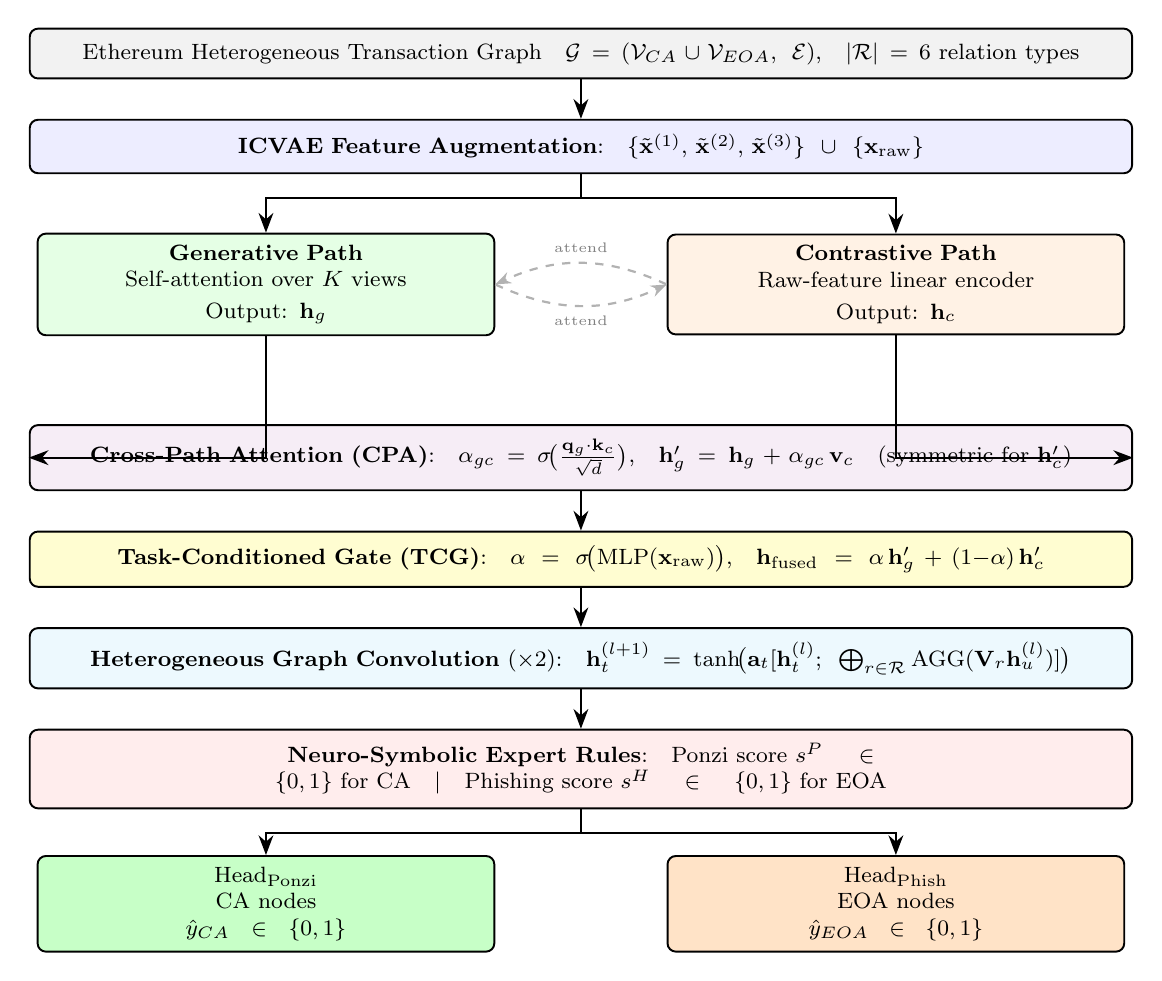
\begin{tikzpicture}[
  Wf/.style={draw, rectangle, rounded corners=3pt, align=center,
             font=\footnotesize, minimum width=14cm,
             text width=13.5cm, inner sep=5pt, line width=0.7pt},
  Hf/.style={draw, rectangle, rounded corners=3pt, align=center,
             font=\footnotesize, minimum width=5.8cm,
             text width=5.5cm, inner sep=4pt, line width=0.7pt},
  SA/.style={-{Stealth[length=2.5mm]}, thick},
  DA/.style={-{Stealth[length=2mm]}, thick, dashed, color=gray!60}
]

% ---- Row 0: input graph ----
\node[Wf, fill=gray!10] (G) at (0,0)
    {Ethereum Heterogeneous Transaction Graph\quad
     $\mathcal{G}=(\mathcal{V}_{CA}\cup\mathcal{V}_{EOA},\;\mathcal{E})$,\quad
     $|\mathcal{R}|=6$ relation types};

% ---- Row 1: ICVAE augmentation ----
\node[Wf, fill=blue!7, below=0.5cm of G] (AUG)
    {\textbf{ICVAE Feature Augmentation}:\quad
     $\{\tilde{\mathbf{x}}^{(1)},\,\tilde{\mathbf{x}}^{(2)},\,\tilde{\mathbf{x}}^{(3)}\}
     \cup\{\mathbf{x}_{\mathrm{raw}}\}$};

% ---- Row 2: dual paths (anchored to AUG.south via calc) ----
\node[Hf, fill=green!10]  (GEN)  at ($(AUG.south)+(-4.0,-1.4)$)
    {\textbf{Generative Path}\\
     Self-attention over $K$ views\\[2pt]
     Output: $\mathbf{h}_g$};

\node[Hf, fill=orange!10] (CONT) at ($(AUG.south)+(4.0,-1.4)$)
    {\textbf{Contrastive Path}\\
     Raw-feature linear encoder\\[2pt]
     Output: $\mathbf{h}_c$};

% ---- Row 3: Cross-Path Attention ----
\node[Wf, fill=violet!7] (CPA) at ($(AUG.south)+(0,-3.6)$)
    {\textbf{Cross-Path Attention (CPA)}:\quad
     $\alpha_{gc}=\sigma\!\bigl(\tfrac{\mathbf{q}_g\cdot\mathbf{k}_c}{\sqrt{d}}\bigr)$,\quad
     $\mathbf{h}'_g=\mathbf{h}_g+\alpha_{gc}\,\mathbf{v}_c$\quad
     (symmetric for $\mathbf{h}'_c$)};

% ---- Row 4: Task-Conditioned Gate ----
\node[Wf, fill=yellow!18, below=0.5cm of CPA] (GATE)
    {\textbf{Task-Conditioned Gate (TCG)}:\quad
     $\alpha=\sigma\!\bigl(\mathrm{MLP}(\mathbf{x}_{\mathrm{raw}})\bigr)$,\quad
     $\mathbf{h}_{\mathrm{fused}}=\alpha\,\mathbf{h}'_g+(1{-}\alpha)\,\mathbf{h}'_c$};

% ---- Row 5: Graph Convolution ----
\node[Wf, fill=cyan!7, below=0.5cm of GATE] (CONV)
    {\textbf{Heterogeneous Graph Convolution} $(\times 2)$:\quad
     $\mathbf{h}^{(l+1)}_t=\tanh\!\bigl(\mathbf{a}_t
     [\mathbf{h}^{(l)}_t;\;
     \bigoplus_{r\in\mathcal{R}}\mathrm{AGG}(\mathbf{V}_r\mathbf{h}^{(l)}_u)]\bigr)$};

% ---- Row 6: Expert Rules ----
\node[Wf, fill=red!7, below=0.5cm of CONV] (EXP)
    {\textbf{Neuro-Symbolic Expert Rules}:\quad
     Ponzi score $s^P\!\in\!\{0,1\}$ for CA\quad$|$\quad
     Phishing score $s^H\!\in\!\{0,1\}$ for EOA};

% ---- Row 7: dual heads (anchored to EXP.south via calc) ----
\node[Hf, fill=green!22] (PH) at ($(EXP.south)+(-4.0,-1.2)$)
    {$\mathrm{Head}_{\mathrm{Ponzi}}$\\ CA nodes\\ $\hat{y}_{CA}\!\in\!\{0,1\}$};

\node[Hf, fill=orange!22] (HH) at ($(EXP.south)+(4.0,-1.2)$)
    {$\mathrm{Head}_{\mathrm{Phish}}$\\ EOA nodes\\ $\hat{y}_{EOA}\!\in\!\{0,1\}$};

% ---- Main flow arrows ----
\draw[SA] (G)    -- (AUG);
\draw[SA] (AUG.south) -- ++(0,-0.3) -| (GEN.north);
\draw[SA] (AUG.south) -- ++(0,-0.3) -| (CONT.north);
\draw[SA] (GEN.south)  -- ++(0,-0.25) |- (CPA.west);
\draw[SA] (CONT.south) -- ++(0,-0.25) |- (CPA.east);
\draw[SA] (CPA)  -- (GATE);
\draw[SA] (GATE) -- (CONV);
\draw[SA] (CONV) -- (EXP);
\draw[SA] (EXP.south) -- ++(0,-0.3) -| (PH.north);
\draw[SA] (EXP.south) -- ++(0,-0.3) -| (HH.north);

% ---- Bidirectional cross-attend (GEN ↔ CONT) ----
\draw[DA] (GEN.east) to[bend right=25]
    node[midway,below,font=\tiny,color=gray]{attend} (CONT.west);
\draw[DA] (CONT.west) to[bend right=25]
    node[midway,above,font=\tiny,color=gray]{attend} (GEN.east);

\end{tikzpicture}
\caption{Overview of the proposed \textbf{UnifiedHMSL} framework.
  ICVAE augmentation generates $K$ stochastic feature views per node.
  A generative path applies self-attention over augmented views while a
  contrastive path encodes raw features directly.
  Cross-Path Attention~(CPA) enables bidirectional information exchange
  between paths; a Task-Conditioned Gate~(TCG) blends the two
  representations adaptively per node type (CA for Ponzi, EOA for phishing).
  Two heterogeneous graph convolution layers propagate fused features;
  Neuro-Symbolic Expert Rules inject domain knowledge before the
  dual classification heads.}
\label{fig:architecture}
\end{figure*}
%----- END FIGURE 1 ---------------------------------------------------

\subsection{Problem Formulation}

Let $\mathcal{G} = (\mathcal{V},\mathcal{E},\phi,\psi)$ be a
heterogeneous graph where $\mathcal{V} = \mathcal{V}_{CA} \cup
\mathcal{V}_{EOA}$ is the node set partitioned into Contract Accounts
and Externally Owned Accounts, $\mathcal{E}$ is the edge set,
$\phi: \mathcal{V}\!\to\!\mathcal{T}$ maps nodes to their types
($|\mathcal{T}|=2$), and $\psi: \mathcal{E}\!\to\!\mathcal{R}$ maps
edges to one of $|\mathcal{R}|=6$ relation types encoding function
calls and value transfers between CA and EOA nodes.

Each CA node $v\in\mathcal{V}_{CA}$ carries a feature vector
$\mathbf{x}_v^{CA}\in\mathbb{R}^{12}$ and a binary Ponzi label
$y_v^P\in\{0,1\}$.  Each EOA node $u\in\mathcal{V}_{EOA}$ carries
a feature vector $\mathbf{x}_u^{EOA}\in\mathbb{R}^d$ and a binary
phishing label $y_u^H\in\{0,1\}$.
The goal is to jointly learn a function
\begin{equation}
  f_\theta:\mathcal{G}
  \;\longrightarrow\;
  \bigl(\hat{\mathbf{y}}^P\in[0,1]^{|\mathcal{V}_{CA}|},\;
         \hat{\mathbf{y}}^H\in[0,1]^{|\mathcal{V}_{EOA}|}\bigr)
\end{equation}
that simultaneously predicts Ponzi and phishing labels with high
macro-F1, under the constraint that fraud instances are rare
($<15\%$ and $<45\%$ respectively).

\subsection{Heterogeneous Graph Construction}

The Ethereum transaction graph is modelled as a heterogeneous graph
with two node types ($CA$, $EOA$) and six directed edge types:
\begin{table}[h]
\centering
\caption{Heterogeneous edge types in the Ethereum transaction graph.}
\label{tab:edges}
\begin{tabular}{@{}ll@{}}
\toprule
Edge relation & Semantics \\
\midrule
$CA \!\to\! EOA$ (call)  & contract calls user \\
$EOA \!\to\! CA$ (call)  & user calls contract \\
$CA \!\to\! CA$ (call)   & inter-contract call \\
$CA \!\to\! EOA$ (trans) & contract transfers to user \\
$EOA \!\to\! CA$ (trans) & user transfers to contract \\
$EOA \!\to\! EOA$ (trans)& user-to-user transfer \\
\bottomrule
\end{tabular}
\end{table}
CA node features encode 12 transaction statistics (e.g.\ total sent,
total received, call balance), while EOA features encode the
corresponding statistics for user accounts.  Raw feature matrices are
stored in $\mathbf{X}^{CA}$ and $\mathbf{X}^{EOA}$.

\subsection{Conditional VAE-based Feature Augmentation}

To address class imbalance, we employ a pre-trained Improved
Conditional Variational Autoencoder (ICVAE)~\cite{li2022graphvae}
that generates synthetic augmented feature views conditioned on source
node features and edge type.

The encoder maps an input node feature $\mathbf{x}$, a condition
vector $\mathbf{c}$ (source neighbourhood features), and an edge-type
one-hot vector $\mathbf{e}$ to a factored Gaussian latent distribution:
\begin{equation}
  \boldsymbol{\mu},\,\log\boldsymbol{\sigma}^2
  = \mathrm{MLP}_{\mathrm{enc}}([\mathbf{x};\mathbf{c};\mathbf{e}]).
\end{equation}
A latent sample is drawn via the reparameterisation trick:
\begin{equation}
  \mathbf{z} = \boldsymbol{\mu} + \boldsymbol{\epsilon}\odot\boldsymbol{\sigma},
  \quad \boldsymbol{\epsilon}\sim\mathcal{N}(\mathbf{0},\mathbf{I}).
\end{equation}
The decoder reconstructs (or synthesises) a node feature view:
\begin{equation}
  \tilde{\mathbf{x}} = \sigma\!\bigl(\mathrm{MLP}_{\mathrm{dec}}([\mathbf{z};\mathbf{c};\mathbf{e}])\bigr).
\end{equation}
At training time we draw $K=3$ independent samples
$\{\tilde{\mathbf{x}}^{(k)}\}_{k=1}^{K}$, producing a multi-view
feature set appended with the original raw features.
The ICVAE is pre-trained separately per task (Ponzi/Phishing) on
the respective training split and kept frozen during GNN training.

\subsection{Multi-Task Dual-Head Architecture}
\label{sec:dualhead}

The original HMSL model~\cite{paper_baseline_2408.00641} produces a
single output via a linear classification head targeting a fixed node
type:
\begin{equation}
\hat{y} = \mathrm{Linear}(\mathbf{h}_{\mathrm{target}}).
\end{equation}
This design requires one trained model per fraud type and prevents
shared representation learning. In contrast, UnifiedHMSL adopts a
dual-head architecture with task-specific output layers:
\begin{equation}
\hat{y}_{\mathrm{Ponzi}} = \mathbf{W}_{\mathrm{Ponzi}}\,
  \mathbf{h}_{CA} + \mathbf{b}_{\mathrm{Ponzi}},
\end{equation}
\begin{equation}
\hat{y}_{\mathrm{Phish}} = \mathbf{W}_{\mathrm{Phish}}\,
  \mathbf{h}_{EOA} + \mathbf{b}_{\mathrm{Phish}}.
\end{equation}
Both heads share a common upstream heterogeneous graph encoder
(node-type projection layers, multi-view attention fusion, and two
heterogeneous graph convolution layers), encouraging transferable
representations of Ethereum transaction patterns.

\subsection{Cross-Path Attention Mechanism}

%----- FIGURE 2: CrossPathAttention detail -------------------------
\begin{figure}[t]
\centering
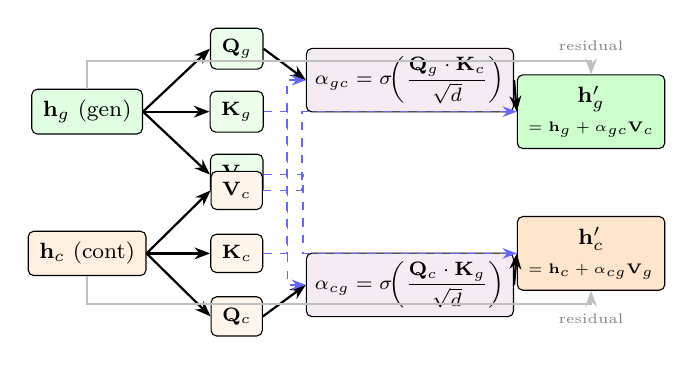
\begin{tikzpicture}[
  IB/.style={draw, rounded corners=2pt, fill=white, align=center,
             font=\footnotesize, inner sep=4pt},
  AB/.style={draw, rounded corners=2pt, fill=violet!8, align=center,
             font=\scriptsize, inner sep=3pt, minimum height=0.7cm},
  OB/.style={draw, rounded corners=2pt, align=center,
             font=\footnotesize, inner sep=4pt},
  SA/.style={-{Stealth[length=2mm]}, thick},
  CA/.style={-{Stealth[length=1.8mm]}, semithick, dashed, blue!60}
]

% Inputs
\node[IB, fill=green!12] (HG)  at (-3.0, 0.9) {$\mathbf{h}_g$ (gen)};
\node[IB, fill=orange!12] (HC) at (-3.0,-0.9) {$\mathbf{h}_c$ (cont)};

% Projection boxes -- gen
\node[IB, fill=green!8]  (Qg) at (-1.1, 1.7) {\scriptsize$\mathbf{Q}_g$};
\node[IB, fill=green!8]  (Kg) at (-1.1, 0.9) {\scriptsize$\mathbf{K}_g$};
\node[IB, fill=green!8]  (Vg) at (-1.1, 0.1) {\scriptsize$\mathbf{V}_g$};

% Projection boxes -- cont
\node[IB, fill=orange!8] (Qc) at (-1.1,-1.7) {\scriptsize$\mathbf{Q}_c$};
\node[IB, fill=orange!8] (Kc) at (-1.1,-0.9) {\scriptsize$\mathbf{K}_c$};
\node[IB, fill=orange!8] (Vc) at (-1.1,-0.1) {\scriptsize$\mathbf{V}_c$};

% Attention score boxes
\node[AB] (AGC) at (1.1, 1.3)
    {$\alpha_{gc}=\sigma\!\!\left(\dfrac{\mathbf{Q}_g\cdot\mathbf{K}_c}{\sqrt{d}}\right)$};
\node[AB] (ACG) at (1.1,-1.3)
    {$\alpha_{cg}=\sigma\!\!\left(\dfrac{\mathbf{Q}_c\cdot\mathbf{K}_g}{\sqrt{d}}\right)$};

% Outputs
\node[OB, fill=green!20, align=center] (HGO) at (3.4, 0.9)
    {$\mathbf{h}'_g$\\[1pt]
     {\tiny$=\mathbf{h}_g+\alpha_{gc}\mathbf{V}_c$}};

\node[OB, fill=orange!20, align=center] (HCO) at (3.4,-0.9)
    {$\mathbf{h}'_c$\\[1pt]
     {\tiny$=\mathbf{h}_c+\alpha_{cg}\mathbf{V}_g$}};

% -- Arrows from inputs to projections --
\draw[SA] (HG.east) -- (Qg.west);
\draw[SA] (HG.east) -- (Kg.west);
\draw[SA] (HG.east) -- (Vg.west);
\draw[SA] (HC.east) -- (Qc.west);
\draw[SA] (HC.east) -- (Kc.west);
\draw[SA] (HC.east) -- (Vc.west);

% -- Cross-attention: Q_g x K_c --> alpha_gc --
\draw[SA] (Qg.east) -- (AGC.west);
\draw[CA] (Kc.east) -- ++(0.3,0) |- (AGC.west);

% -- Cross-attention: Q_c x K_g --> alpha_cg --
\draw[SA] (Qc.east) -- (ACG.west);
\draw[CA] (Kg.east) -- ++(0.3,0) |- (ACG.west);

% -- alpha_gc * V_c --> h'_g --
\draw[SA] (AGC.east) -- (HGO.west);
\draw[CA] (Vc.east) -- ++(0.5,0) |- (HGO.west);

% -- alpha_cg * V_g --> h'_c --
\draw[SA] (ACG.east) -- (HCO.west);
\draw[CA] (Vg.east) -- ++(0.5,0) |- (HCO.west);

% Residual connection labels
\draw[SA, gray!50] (HG.north) -- ++(0,0.35) -| (HGO.north)
    node[midway, above, font=\tiny, color=gray] {residual};
\draw[SA, gray!50] (HC.south) -- ++(0,-0.35) -| (HCO.south)
    node[midway, below, font=\tiny, color=gray] {residual};

\end{tikzpicture}
\caption{Cross-Path Attention (CPA) module. The generative path
  $\mathbf{h}_g$ queries the contrastive path's keys $\mathbf{K}_c$
  to produce a gated attention weight $\alpha_{gc}$, then absorbs the
  contrastive path's values $\mathbf{V}_c$ via a residual connection.
  The symmetric operation updates $\mathbf{h}_c$ using
  $\mathbf{K}_g$ and $\mathbf{V}_g$.
  Dashed blue arrows indicate cross-path information flow.}
\label{fig:cpa}
\end{figure}
%----- END FIGURE 2 -----------------------------------------------

Fig.~\ref{fig:cpa} depicts the Cross-Path Attention module.
Given the generative representation $\mathbf{h}_g$ and the contrastive
representation $\mathbf{h}_c$ for nodes of a given type, the module
computes two mutual gated updates.

The generative path attends to the contrastive path:
\begin{equation}
  \alpha_{gc} = \sigma\!\left(
    \frac{\bigl(\mathbf{W}^Q_g\,\mathbf{h}_g\bigr)
          \odot
          \bigl(\mathbf{W}^K_c\,\mathbf{h}_c\bigr)}
         {\sqrt{d}}
  \right),
  \label{eq:alpha_gc}
\end{equation}
\begin{equation}
  \mathbf{h}'_g = \mathbf{h}_g +
    \alpha_{gc} \odot \mathrm{Dropout}\!\bigl(\mathbf{W}^V_c\,\mathbf{h}_c\bigr).
  \label{eq:hg_prime}
\end{equation}
Symmetrically, the contrastive path attends to the generative path:
\begin{equation}
  \alpha_{cg} = \sigma\!\left(
    \frac{\bigl(\mathbf{W}^Q_c\,\mathbf{h}_c\bigr)
          \odot
          \bigl(\mathbf{W}^K_g\,\mathbf{h}_g\bigr)}
         {\sqrt{d}}
  \right),
  \label{eq:alpha_cg}
\end{equation}
\begin{equation}
  \mathbf{h}'_c = \mathbf{h}_c +
    \alpha_{cg} \odot \mathrm{Dropout}\!\bigl(\mathbf{W}^V_g\,\mathbf{h}_g\bigr).
  \label{eq:hc_prime}
\end{equation}
The sigmoid gate (rather than softmax) in
Eqs.~\eqref{eq:alpha_gc}--\eqref{eq:alpha_cg} produces
element-wise attention weights in $(0,1)$, enabling the model to
selectively suppress irrelevant cross-path signals.
The residual connection in Eqs.~\eqref{eq:hg_prime}--\eqref{eq:hc_prime}
preserves each path's own signal, so CPA is an \emph{additive} refinement
rather than a replacement.  Separate CPA modules are maintained for
CA and EOA node types.

\subsection{Task-Conditioned Gating}

After CPA, each node type has updated representations $\mathbf{h}'_g$
and $\mathbf{h}'_c$.  Rather than combining them with a fixed weight,
the Task-Conditioned Gate (TCG) learns a node-level blending coefficient
from the original raw features:
\begin{equation}
  \alpha = \sigma\!\bigl(
    \mathbf{W}_2\,\mathrm{ReLU}(\mathbf{W}_1\,\mathbf{x}_{\mathrm{raw}})
  \bigr) \;\in\; (0,1)^{N\times 1},
  \label{eq:gate}
\end{equation}
\begin{equation}
  \mathbf{h}_{\mathrm{fused}} = \alpha \odot \mathbf{h}'_g
    + (1-\alpha) \odot \mathbf{h}'_c.
  \label{eq:fused}
\end{equation}
By conditioning the gate on $\mathbf{x}_{\mathrm{raw}}$, the model
can weight the augmented generative path more heavily for nodes where
augmentation is reliable, and fall back to the raw contrastive path
for nodes where CVAE generation is uncertain.
Crucially, \emph{separate} TCG modules are used for CA and EOA node
types, allowing the Ponzi task and the phishing task to develop
distinct blending strategies from the same underlying feature space.

\subsection{Neuro-Symbolic Integration (Expert Rules)}
\label{sec:expert}

To inject domain knowledge into the neural pipeline we define
two symbolic scoring functions derived from on-chain transaction
anomaly patterns.

\medskip\noindent\textbf{Ponzi score.}
A CA node is flagged by expert rule $s^P\!\in\!\{0,1\}$ if it
exhibits a known Ponzi redistribution signature:
\begin{equation}
  s^P = \mathbf{1}\!\left[
    \bigl(\mathbf{x}^{CA}_{7} > 0\bigr)
    \wedge
    \bigl(\mathbf{x}^{CA}_{4} \le 3.5 \;\vee\; \mathbf{x}^{CA}_{11} > 269.0\bigr)
  \right]
  \;\vee\;
  \mathbf{1}\!\left[
    \mathbf{x}^{CA}_{7}\le 0 \wedge \mathbf{x}^{CA}_{0} > 10
  \right],
\end{equation}
where $\mathbf{x}^{CA}_{0},\mathbf{x}^{CA}_{4},\mathbf{x}^{CA}_{7},
\mathbf{x}^{CA}_{11}$ denote call total sent, call balance, transfer
total sent, and transfer balance respectively.

\medskip\noindent\textbf{Phishing score.}
An EOA node is flagged by expert rule $s^H\!\in\!\{0,1\}$ under two
complementary conditions:
\begin{equation}
  s^H = \mathbf{1}\!\left[
    \mathbf{x}^{EOA}_{8} \le 102.04
    \wedge \mathbf{x}^{EOA}_{7} > {-10}
    \wedge \mathbf{x}^{EOA}_{0} > {-12.75}
  \right]
  \;\vee\;
  \mathbf{1}\!\left[
    \mathbf{x}^{EOA}_{8} > 150 \wedge s_{\mathrm{whale}}
  \right],
\end{equation}
where the whale condition $s_{\mathrm{whale}}$ captures high-deposit
accounts with zero call activity---a common pattern among dormant
phishing wallets.

\medskip\noindent\textbf{Integration modes.}
Expert scores are incorporated in one of two modes controlled by
hyperparameter \texttt{expert\_mode}:
\begin{itemize}
\item \textbf{Feature mode}: $s^P$ (resp.\ $s^H$) is appended as an
  extra input dimension to the CA (resp.\ EOA) node representation
  before the classification head:
  $\mathbf{h}^{\mathrm{final}}_{CA} = [\mathbf{h}_{CA}; s^P]$.
\item \textbf{Loss mode}: expert scores serve as soft targets in an
  auxiliary MSE loss that penalises disagreement between the neural
  prediction and the symbolic score, without modifying the feature
  space.
\end{itemize}

\subsection{Contrastive Self-Supervision via Triplet Loss}

The $K$ stochastic ICVAE views also serve as positive and negative
samples for contrastive self-supervision.  For each node type we
construct triplets from the augmented embedding list
$\{\mathbf{z}^{(1)},\mathbf{z}^{(2)},\mathbf{z}^{(3)}\}$ by
designating:
\begin{equation}
  \mathbf{a} = \mathbf{z}^{(2)},\quad
  \mathbf{p} = \mathbf{z}^{(3)},\quad
  \mathbf{n} = \mathbf{z}^{(1)}.
\end{equation}
The triplet contrastive loss (with self-attention aggregation over the
embedding sequence) is:
\begin{equation}
  \mathcal{L}_{\mathrm{tri}} =
    \max\!\bigl(
      \|\mathbf{a}-\mathbf{p}\|^2 - \|\mathbf{a}-\mathbf{n}\|^2
      + \delta,\; 0
    \bigr),
  \quad \delta = 0.3.
\end{equation}
The loss encourages consecutive stochastic views of the same node to
be closer in embedding space than non-consecutive ones, promoting
compact, discriminative representations.

\subsection{Training Objective}

The full joint loss is:
\begin{equation}
  \mathcal{L}
  = \underbrace{
      \mathcal{L}_{\mathrm{CE}}^{P}
      + \mathcal{L}_{\mathrm{CE}}^{H}
    }_{\text{task supervision}}
  + \;\lambda\underbrace{
      \bigl(\mathcal{L}_{\mathrm{tri}}^{CA}
       + \mathcal{L}_{\mathrm{tri}}^{EOA}\bigr)
    }_{\text{contrastive}}
  + \;\frac{1}{2}\underbrace{
      \bigl(\mathcal{L}_{\mathrm{exp}}^{P}
       + \mathcal{L}_{\mathrm{exp}}^{H}\bigr)
    }_{\text{expert (loss mode)}},
  \label{eq:loss}
\end{equation}
where $\mathcal{L}_{\mathrm{CE}}^{P}$ and $\mathcal{L}_{\mathrm{CE}}^{H}$
are cross-entropy losses for Ponzi and phishing classification,
$\mathcal{L}_{\mathrm{tri}}^{CA/EOA}$ are node-type-specific triplet
losses, $\mathcal{L}_{\mathrm{exp}}^{P/H}$ are MSE losses between
model outputs and expert scores (active only when
\texttt{expert\_mode}$=$\texttt{loss}), and $\lambda=0.1$ is a
balancing hyperparameter.

%-------------------------------------------------------------------
\section{Experiments and Evaluation}
\label{sec:experiments}

\subsection{Datasets}
We evaluate UnifiedHMSL on two Ethereum transaction graph datasets:

\noindent\textbf{Ponzi Dataset.}
Contains $1{,}342$ CA nodes ($191$ Ponzi, $1{,}151$ legitimate)
and their associated EOA neighbours, connected by the six edge types
described in Section~\ref{sec:methodology}.
Each CA node is described by 12 transaction statistics.
The severe class imbalance ratio is approximately $1{:}6$.

\noindent\textbf{Phishing Dataset.}
Contains $2{,}763$ EOA nodes ($1{,}206$ phishing, $1{,}557$ legitimate)
and their associated CA neighbours.
The class imbalance ratio is approximately $1{:}1.3$.

Both datasets share the same heterogeneous graph topology: CA and EOA
nodes are co-present and connected by the same six edge types.
Data splits follow a $60\%/20\%/20\%$ train/validation/test partition
stratified by label.

\subsection{Experimental Setup}
All experiments are conducted on a single GPU (NVIDIA RTX series).
The GNN hidden dimension is set to $128$, the learning rate to
$0.001$, the batch size to $512$, and training runs for up to
$1{,}000$ epochs with early stopping (patience $= 100$) based on
the sum of macro-F1 scores on the validation set.
NeighborLoader samples $100$ neighbours per hop for two hops.
The contrastive loss weight is $\lambda = 0.1$ and the CVAE latent
dimension is $32$.  Expert rules are applied in \textbf{feature}
mode (\texttt{expert\_mode}$=$\texttt{feature}) by default.

Macro-F1 is the primary evaluation metric, as it accounts for class
imbalance by averaging per-class F1 scores.

\subsection{Computational Cost and Model Stability}
The dual-task architecture introduces marginal overhead compared to
running two single-task models: the shared encoder is trained once,
and the additional CPA and TCG modules add $\mathcal{O}(d^2)$
parameters per node type.  Model training is stable across random
seeds due to the three-view CVAE augmentation, which reduces variance
in minority-class representations.  Convergence is monitored via the
sum of validation macro-F1 scores across both tasks.

\subsection{Results and Discussion}

\textit{[Results table and analysis to be inserted after experimental
runs are completed.]}

%-------------------------------------------------------------------
\section{Conclusion}
\label{sec:conclusion}

We presented \textbf{UnifiedHMSL}, a unified multi-task heterogeneous
GNN for simultaneous Ponzi scheme and phishing scam detection on the
Ethereum transaction graph.  The framework integrates four key
innovations: a pre-trained ICVAE for stochastic multi-view feature
augmentation, a Cross-Path Attention module for mutual generative--contrastive
information exchange, a Task-Conditioned Gate for adaptive per-node-type
feature blending, and a neuro-symbolic Expert Rules module for
domain-knowledge injection.  These components are trained jointly under
a combined cross-entropy, triplet contrastive, and expert-guided loss.

The unified architecture enables shared representation learning between
Ponzi and phishing detection tasks while remaining computationally
efficient.  Future work will explore dynamic graph settings, where node
features and topology evolve over time, and extend the expert rule
framework to include mined transaction pattern rules learned from
historical fraud cases.

%-------------------------------------------------------------------
\bibliographystyle{IEEEtran}
\bibliography{references}

\end{document}
